%% Requires compilation with XeLaTeX or LuaLaTeX
\documentclass[10pt,xcolor={table,dvipsnames},t]{beamer}
\usetheme{UCBerkeley}

\title[Your Short Title]{Solving 2D problems}
\subtitle{Your subtitle (if there's one)}
\author{Bhanu Prakash \\Yaswanth}
\institute{electrical}
\date{Date of Presentation:14 feb 2019}

\begin{document}

\begin{frame}
  \titlepage
\end{frame}

% Uncomment these lines for an automatically generated outline.
%\begin{frame}{Outline}
%  \tableofcontents
%\end{frame}

\section{Introduction}

\begin{frame}{geometric question}

\begin{itemize}
  \item Given,the axis of the ellipse are the co-ordinate axes and passes through points(2,-1) and(4,-2).find the eccentricity.
  \item  \texttt{} 
\end{itemize}




\end{frame}

\section{Some \LaTeX{} Examples}

\subsection{Mathematics}

\begin{frame}{Geometry question into matrix formation}
The ellipse passes through the point P=
\begin{bmatrix}
 4 \\
 -1
\end{bmatrix}
and Q=
\begin{bmatrix}
 -2 \\
 2
\end{bmatrix}
then find the eccentricity of the ellipse.
\end{frame}


\subsection{Tables and Figures}

\smallframetitle

\begin{frame}{Solution using matrices}



\begin{itemize}
Given P=
\begin{bmatrix}
 4 \\
 -1
 
\end{bmatrix}
and Q=
\begin{bmatrix}
 -2 \\
 2
\end{bmatrix}
The ellipse equation is
\begin{equation}
    x^2/a^2+y^2/b^2=1
\end{equation}
By substituting P,Q points in the ellipse equation we get a,b.
By this a=4.47 and
b=2.23
then 
\begin{equation}
    c=b/a = 0.498
\end{equation}
then eccentricity
\begin{equation}
    e=\sqrt(1-b^2/a^2)=0.867
\end{equation}


\end{itemize}



\end{frame}

\begin{frame}
\frametitle{Plot}
\begin{figure}
    \centering
    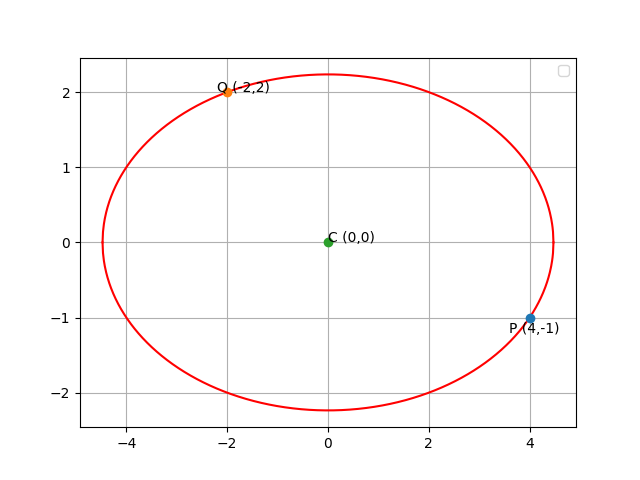
\includegraphics[scale=0.5]{Figure.png}
\end{figure}
Commands to include a figure:

\begin{figure}
\includegraphics[width=0.4\textwidth]{chart}
\caption{\label{fig:your-figure}Caption goes here.}
\end{figure}
\end{frame}





\end{document}
